\documentclass{beamer}

\usetheme{LMU}

\usepackage[utf8]{inputenc}
\usepackage[T1]{fontenc}

\usepackage[english]{babel}
\usepackage{url}
%\usepackage{cite}
%\usepackage{natbib}
\usepackage[backend=bibtex,style=authoryear,dashed=false]{biblatex}
\addbibresource{../bib/eigene.bib}
\addbibresource{../bib/itip-refs.bib}
\addbibresource{../bib/other-refs.bib}
\renewcommand{\bibfont}{\normalfont\scriptsize}
\setlength{\bibhang}{3ex}

\usepackage{amssymb, amsmath, amsfonts, enumerate}
%\usepackage{bbold}
\newcommand\hmmax{0}
\usepackage{bm}
%\usepackage{dsfont}
\usepackage{pxfonts}
\usepackage{xcolor}

\usepackage{tikz}
\usetikzlibrary{%
   arrows,%
   calc,%
   fit,%
   patterns,%
   plotmarks,%
   shapes.geometric,%
   shapes.misc,%
   shapes.symbols,%
   shapes.arrows,%
   shapes.callouts,%
   shapes.multipart,%
   shapes.gates.logic.US,%
   shapes.gates.logic.IEC,%
   er,%
   automata,%
   backgrounds,%
   chains,%
   topaths,%
   trees,%
   petri,%
   mindmap,%
   matrix,%
   calendar,%
   folding,%
   fadings,%
   through,%
   patterns,%
   positioning,%
   scopes,%
   decorations.fractals,%
   decorations.shapes,%
   decorations.text,%
   decorations.pathmorphing,%
   decorations.pathreplacing,%
   decorations.footprints,%
   decorations.markings,%
   shadows,%
   spy}
%\usepackage{bbold}
\usepackage{hyperref}

\setbeamertemplate{blocks}[rounded][shadow=true]
\definecolor{lmugreen2}{RGB}{0,120,94}
%\definecolor{lmugreen2}{RGB}{0,148,64}
\definecolor{lmugreen}{RGB}{0,140,84}
\definecolor{unidurham}{RGB}{126,49,123}

\parindent0pt
\setlength{\unitlength}{1ex}
\setlength{\fboxsep}{0ex}

\def\then{{\color{lmugreen}$\rule[0.35ex]{2ex}{0.5ex}\!\!\!\blacktriangleright$}}
%\def\then{{\color{lmugreen}$\blacktriangleright\!\blacktriangleright$}}
%\def\then{{\color{lmugreen}$\blacktriangleright$}}
%\def\then{{\color{lmugreen}$\Rrightarrow$}}
%\def\then{{\color{lmugreen}$\rhd$}}
%\def\then{{\color{lmugreen}$\gg\!\!\!\!\!\gg$}}
%\def\then{{\color{lmugreen}${\mathbf{\gg}}$}}
\def\play{{\color{lmugreen}$\blacktriangleright$}}

\def\rthen{{\color{lmugreen}$\rule[0.35ex]{0.5ex}{0.95ex}\rule[0.35ex]{1.3ex}{0.5ex}\!\!\!\blacktriangleright$}}

\def\thenthen{{\color{lmugreen}$\blacktriangleleft\!\!\!\rule[0.35ex]{2ex}{0.5ex}\!\!\!\blacktriangleright$}}

\def\gplus{{\color{lmugreen}\rule[0.45ex]{1.4ex}{0.4ex}\hspace{-0.9ex}\rule[0.0ex]{0.4ex}{1.3ex}\hspace{0.5ex}}}
\def\gminus{{\color{lmugreen}\rule[0.45ex]{1.4ex}{0.4ex}}}


\def\blau#1{{\color{lmugreen2}#1}}
\def\rot#1{{\color{red}#1}}
\def\gruen#1{{\color{blue}#1}}
%\def\gruen#1{{\color{gray}#1}}

%%%%%%%%%%%%%%%%%%%%%%%%%%%%%%%%%%%%%%%%%
%% Definitions & shortcuts for thesis  %%
%%%%%%%%%%%%%%%%%%%%%%%%%%%%%%%%%%%%%%%%%

\def\pdc{prior-data conflict}

\newcommand{\reals}{\mathbb{R}}

\newcommand{\dd}{\,\mathrm{d}}

\newcommand{\mbf}[1]{\mathbf{#1}}

\newcommand{\X}{\mbf{X}}
\newcommand{\x}{\mbf{x}}

\def\yzr{\rot{\yz}}
\def\ynr{\rot{\yn}}
\def\byzr{\rot{\byz}}
\def\bynr{\rot{\byn}}
\def\yzor{\rot{y\uz_1}}
\def\yzjr{\rot{y\uz_j}}
\def\yzkr{\rot{y\uz_k}}
\def\yzlr{\rot{\yzl}}
\def\yzur{\rot{\yzu}}
\def\ynjr{\rot{y\un_j}}
\def\ynlr{\rot{\ynl}}
\def\ynur{\rot{\ynu}}
\def\yzjlr#1{\rot{\ul{y}\uz_#1}}
\def\yzjur#1{\rot{\ol{y}\uz_#1}}


\def\nzg{\gruen{\nz}}
\def\nng{\gruen{\nn}}
\def\nzlg{\gruen{\nzl}}
\def\nzug{\gruen{\nzu}}
\def\nnlg{\gruen{\nnl}}
\def\nnug{\gruen{\nnu}}

\def\psib{\blau{\psi}}
\def\bpsib{\blau{{b}(\psi)}}


% ------------ shading start
\newsavebox{\tempbox}
\newcommand\leftrightshading[3]{%
  \begin{tikzfadingfrompicture}[name=inputtext]
    \node [text=white] {#1};
  \end{tikzfadingfrompicture}
  \begin{lrbox}{\tempbox}%
    \begin{tikzpicture}
      \node [text=white,inner sep=0pt,outer sep=0pt] (textnode) {#1};
      \shade[path fading=inputtext,fit fading=false,left color=#2,right color=#3]
      (textnode.south west) rectangle (textnode.north east);
    \end{tikzpicture}%
  \end{lrbox}
  % Now we use the fading in another picture:
  \usebox\tempbox{}%
}
% ------------ shading end


%\def\PZc{\mathrm I\!\Pi\uz}
\def\PZc{\leftrightshading{$\mathrm I\!\Pi\uz$}{blue}{red}}
%\def\PNc{\PN}
\def\PNc{\leftrightshading{$\mathrm I\!\Pi\un$}{blue}{red}}


\title[Generalised Bayesian Inference \& Prior-Data Conflict]
{Generalised Bayesian Inference\\ under Prior-Data Conflict}

\author%[]
       {Gero Walter}

\institute{Department of Statistics\\
           Ludwig-Maximilians-Universit\"at M\"unchen (LMU)\\
                      {}%\{gero.walter; thomas\}@stat.uni-muenchen.de
}

\date{October 25th, 2013}


\titlegraphic{
%\begin{center}

\includegraphics[scale=0.032]{lmu_logos/lmu_massiv.png}
\raisebox{1.375cm}{
\includegraphics[scale=0.4]{lmu_logos/lmu_statistic.pdf}
}
%\end{center}
}

%---- Notes ---------------------
\setbeameroption{hide notes}
%\setbeameroption{show only notes}

\begin{document}


\frame{
\titlepage
}

% ---------- brace with label -----------
%\draw[decorate,decoration={brace,mirror,raise=5pt},blue]
%\draw[thick,decorate,decoration=brace] (2.2,-1.5) -- (2.2,-2.7) node[midway,right,align=left] %
%{motivating example:\\ {\color{lmugreen} common-cause failure}};

\frame{\frametitle{Overview}
\begin{tikzpicture}%[spy using outlines={rectangle, magnification=3, size=1.5cm, connect spies}]
\path (-1.5,-5) rectangle (10.5,2);
\node[draw] at (0,0) {\includegraphics[scale=0.12]{../diss-toc-1.pdf}};
\node[draw] at (3,0) {\includegraphics[scale=0.12]{../diss-toc-2.pdf}};
\node[draw] at (6,0) {\includegraphics[scale=0.12]{../diss-toc-3.pdf}};
\node[draw] at (9,0) {\includegraphics[scale=0.12]{../diss-toc-4.pdf}};
\end{tikzpicture}
}

% page 1
\addtocounter{framenumber}{-1} 
\frame{\frametitle{Overview}
\begin{tikzpicture}%[spy using outlines={rectangle, magnification=3, size=1.5cm, connect spies}]
\path (-1.5,-5) rectangle (10.5,2);
\node[draw, yellow!60!red, fill=white!60!yellow] at (0,0) {\includegraphics[scale=0.12]{../diss-toc-1.pdf}};
\node[draw] at (3,0) {\includegraphics[scale=0.12]{../diss-toc-2.pdf}};
\node[draw] at (6,0) {\includegraphics[scale=0.12]{../diss-toc-3.pdf}};
\node[draw] at (9,0) {\includegraphics[scale=0.12]{../diss-toc-4.pdf}};
%
\node[draw, yellow!60!red, fill=white] at (1.3,-1.5) {\includegraphics[scale=0.225]{../diss-toc-1.pdf}};
\end{tikzpicture}
}

\addtocounter{framenumber}{-1} 
\frame{\frametitle{Overview}
\begin{tikzpicture}[spy using outlines={rectangle, magnification=3, width=11cm, connect spies}]
\path (-1.5,-5) rectangle (10.5,2);
\node[draw, yellow!60!red, fill=white!60!yellow] at (0,0) {\includegraphics[scale=0.12]{../diss-toc-1.pdf}};
\node[draw] at (3,0) {\includegraphics[scale=0.12]{../diss-toc-2.pdf}};
\node[draw] at (6,0) {\includegraphics[scale=0.12]{../diss-toc-3.pdf}};
\node[draw] at (9,0) {\includegraphics[scale=0.12]{../diss-toc-4.pdf}};
\node[draw, yellow!60!red, fill=white] at (1.3,-1.5) {\includegraphics[scale=0.225]{../diss-toc-1.pdf}};
\spy[red, height=0.55cm] on (1.34,-1.3) in node [fill=white] at (5, 1.5);
\end{tikzpicture}
}

\addtocounter{framenumber}{-1} 
\frame{\frametitle{Overview}
\begin{tikzpicture}[spy using outlines={rectangle, magnification=3, width=11cm, connect spies}]
\path (-1.5,-5) rectangle (10.5,2);
\node[draw, yellow!60!red, fill=white!60!yellow] at (0,0) {\includegraphics[scale=0.12]{../diss-toc-1.pdf}};
\node[draw] at (3,0) {\includegraphics[scale=0.12]{../diss-toc-2.pdf}};
\node[draw] at (6,0) {\includegraphics[scale=0.12]{../diss-toc-3.pdf}};
\node[draw] at (9,0) {\includegraphics[scale=0.12]{../diss-toc-4.pdf}};
\node[draw, yellow!60!red, fill=white] at (1.3,-1.5) {\includegraphics[scale=0.225]{../diss-toc-1.pdf}};
\spy[red, height=0.55cm] on (1.34,-1.3) in node [fill=white] at (5, 1.5);
\spy[red, height=3.55cm] on (1.34,-3.4) in node [fill=white] at (5,-0.8);
\end{tikzpicture}
}

% page 2
\addtocounter{framenumber}{-1} 
\frame{\frametitle{Overview}
\begin{tikzpicture}%[spy using outlines={rectangle, magnification=3, size=1.5cm, connect spies}]
\path (-1.5,-5) rectangle (10.5,2);
\node[draw] at (0,0) {\includegraphics[scale=0.12]{../diss-toc-1.pdf}};
\node[draw, yellow!60!red, fill=white!60!yellow] at (3,0) {\includegraphics[scale=0.12]{../diss-toc-2.pdf}};
\node[draw] at (6,0) {\includegraphics[scale=0.12]{../diss-toc-3.pdf}};
\node[draw] at (9,0) {\includegraphics[scale=0.12]{../diss-toc-4.pdf}};
%
\node[draw, yellow!60!red, fill=white] at (1.3,-1.5) {\includegraphics[scale=0.225]{../diss-toc-2.pdf}};
\end{tikzpicture}
}

% page 3
\addtocounter{framenumber}{-1} 
\frame{\frametitle{Overview}
\begin{tikzpicture}%[spy using outlines={rectangle, magnification=3, size=1.5cm, connect spies}]
\path (-1.5,-5) rectangle (10.5,2);
\node[draw] at (0,0) {\includegraphics[scale=0.12]{../diss-toc-1.pdf}};
\node[draw] at (3,0) {\includegraphics[scale=0.12]{../diss-toc-2.pdf}};
\node[draw, yellow!60!red, fill=white!60!yellow] at (6,0) {\includegraphics[scale=0.12]{../diss-toc-3.pdf}};
\node[draw] at (9,0) {\includegraphics[scale=0.12]{../diss-toc-4.pdf}};
%
\node[draw, yellow!60!red, fill=white] at (1.3,-1.5) {\includegraphics[scale=0.225]{../diss-toc-3.pdf}};
\end{tikzpicture}
}

% page 4
\addtocounter{framenumber}{-1} 
\frame{\frametitle{Overview}
\begin{tikzpicture}%[spy using outlines={rectangle, magnification=3, size=1.5cm, connect spies}]
\path (-1.5,-5) rectangle (10.5,2);
\node[draw] at (0,0) {\includegraphics[scale=0.12]{../diss-toc-1.pdf}};
\node[draw] at (3,0) {\includegraphics[scale=0.12]{../diss-toc-2.pdf}};
\node[draw] at (6,0) {\includegraphics[scale=0.12]{../diss-toc-3.pdf}};
\node[draw, yellow!60!red, fill=white!60!yellow] at (9,0) {\includegraphics[scale=0.12]{../diss-toc-4.pdf}};
%
\node[draw, yellow!60!red, fill=white] at (1.3,-1.5) {\includegraphics[scale=0.225]{../diss-toc-4.pdf}};
\end{tikzpicture}
}


\iffalse
% ----------------------------------------fast-forward compiling
\section{Common-cause Failure Modelling}
\subsection{Alpha-Factor Model}
\subsection{Bayesian Inference}
\subsection{Imprecise Dirichlet Model}
\frame{
Outline of the talk***
\begin{enumerate}
\item Bayesian inference \& prior-data conflict %and Strong prior-data agreement
\item Generalised Bayesian inference with sets of priors\\ (joint work with Thomas Augustin and Frank Coolen)
\item Common-cause failure modeling\\ (joint work with Matthias Troffaes and Dana Kelly)
\end{enumerate}
}
\end{document}
% ----------------------------------------fast-forward compiling
\fi


\frame{\frametitle{Overview}
%Outline of the talk***
\begin{enumerate}
\item Bayesian inference \& prior-data conflict %and Strong prior-data agreement
\item Generalised Bayesian inference with sets of priors\\ (joint work with Thomas Augustin and Frank Coolen)
\item Common-cause failure modeling\\ (joint work with Matthias Troffaes and Dana Kelly)
\end{enumerate}
}

\iffalse
\frame{\frametitle{Overview}
\begin{enumerate}
\item Introduction
 \begin{enumerate}
 \item Preliminaries
 \item Some Fundamentals
 \item Dirichlet-Multinomial Model for Common-Cause Failure
 \end{enumerate}
\item Imprecise Probability as Foundation of Generalised Bayesian Inference
 \begin{enumerate}
 \item Imprecise or Interval Probability
 \item Motives for the Use of Imprecise Probability
 \end{enumerate}
\item Generalised Bayesian Inference with Sets of Conjugate Priors in Exponential Families
 \begin{enumerate}
 \item Model Overview and Discussion
 \item Alternative Models Using Sets of Priors
 \item Imprecision and Prior-Data Conflict in Generalised Bayesian Inference
 \item The \texttt{luck} Package
 \item On Prior-Data Conflict inPredictive Bernoulli Inferences
 \end{enumerate}
\end{enumerate}
}

\frame{\frametitle{Overview}
\begin{enumerate}
\item[4.] Concluding Remarks
 \begin{enumerate}
 \item[4.1] Summary
 \item[4.2] Discussion
 \item[4.3] Outlook
 \end{enumerate}
\item[A.] Appendix
 \begin{enumerate}
 \item[A.1] Bayesian Linear Regression: Different Conjugate Models and Their (In)Sensitivity to Prior-Data Conflict
 \item[A.2] A Parameter Set Shape for Strong Prior-Data Agreement Modelling
 \end{enumerate}
\end{enumerate}

Outline of the talk***
\begin{enumerate}
\item Bayesian inference \& prior-data conflict %and Strong prior-data agreement
\item Generalised Bayesian inference with sets of priors\\ (joint work with Thomas Augustin and Frank Coolen)
\item Common-cause failure modeling\\ (joint work with Matthias Troffaes and Dana Kelly)
\end{enumerate}
}
\fi

\section{Bayesian Inference \& Prior-Data Conflict}

\subsection{Bayesian Inference}

\frame{\frametitle{Bayesian Inference \& Prior-Data Conflict}

\uncover<1->{%
\begin{block}{The Bayesian approach to statistical inference}
\centerline{prior $p(\vartheta)$ + likelihood $f(\x\mid\vartheta)$\hspace*{1ex} \then\ \ posterior $p(\vartheta\mid\x)$}
%\quad using Bayes' Rule}
All inferences are based on the posterior (e.g., point estimate, \ldots)
\end{block}}
\uncover<2->{%
Assigning a certain prior distribution on $\vartheta$\\
\hfill $=$ defining a conglomerate of probability statements (on $\vartheta$)
}
\uncover<3->{%
\begin{block}{Prior-Data Conflict}
\begin{itemize}
\item \emph{informative prior beliefs} and \emph{trusted data}\\ %\rule{0ex}{3ex}\\
(sampling model correct, no outliers, etc.) are in conflict%\\%[2ex]
\item ``[\ldots] the prior [places] its mass primarily on distributions
in the sampling model for which the observed data is surprising''\\
(Evans \& Moshonov, 2006)
\item there are not enough data to overrule the prior
\end{itemize}
\end{block}}
\note<3>[item]{real-world example where \pdc\ is relevant at the end of the talk}
}


\frame{\frametitle{Prior-Data Conflict: Basic Example}

%Example Beta-Binom, show point, line, rectangle
\begin{itemize}[<+->]
\item Bernoulli observations: 0/1 observations (team wins no/yes)
\item given: a set of observations and strong prior information
%\item given: a set of observations (team won 12 out of 16 matches)
%\item additional to observations, we have strong prior information\\ (we are convinced that $P(\text{win})$ should be around $0.75$)
\item we are, e.g., interested in (predictive) probability $P$ that team wins in the next match
%(or some other inferences) %(predictive probability!)
%\item standard statistical model for this situation: Beta-Bernoulli/Binomial Model
%\item \textbf{\pdc:} if $P(\text{heads})$ for the coin is actually very different from our prior guess
%(i.e., prior information and data are in conflict), this should show up in the %predictive
%inferences (probability $\mbox{P}$ and, e.g., confidence intervals)
\end{itemize}
\uncover<4->{
\begin{block}{Beta-Binomial Model}
\begin{tabular}{r|lcl}
data :           & $s\mid \theta$          & $\sim$ & $\bin(n,\theta)$   \\[0.5ex]
conjugate prior: & $\theta\mid \nzg, \yzr$ & $\sim$ & $\be(\nzg,\, \yzr)$  \\[0.5ex]
\cline{1-4}
posterior:       & $\theta\mid \nng, \ynr$ & $\sim$ & $\be(\nng,\, \ynr)$\rule{0ex}{2.5ex}
%\quad ($\frac{\tau(\x)}{n} = \frac{s}{n}$)\rule{0ex}{2.5ex}
\end{tabular}
\end{block}
where $s$ = number of wins in the $n$ matches observed
}
}

\subsection{Example: Beta-Binomial Model}

\frame{\frametitle{Beta-Binomial Model}

\uncover<1->{
\begin{block}{Beta-Binomial Model}
\begin{tabular}{r|lcl}
data :           & $s\mid \theta$          & $\sim$ & $\bin(n,\theta)$   \\[0.5ex]
conjugate prior: & $\theta\mid \nzg, \yzr$ & $\sim$ & $\be(\nzg,\, \yzr)$  \\[0.5ex]
\cline{1-4}
posterior:       & $\theta\mid \nng, \ynr$ & $\sim$ & $\be(\nng,\, \ynr)$\rule{0ex}{2.5ex}
%\quad ($\frac{\tau(\x)}{n} = \frac{s}{n}$)\rule{0ex}{2.5ex}
\end{tabular}
\end{block}
}
\begin{align*}
\uncover<2->{%
P = \E[\theta\mid\nng,\ynr]
}%
\uncover<3->{%
= \rot{\yn}
= \frac{\gruen{\nz}}{\gruen{\nz} + n} \cdot \rot{\yz} + \frac{n}{\gruen{\nz} + n} \cdot \frac{s}{n}
}%
\end{align*}\vspace*{-3ex}
\begin{align*}
\uncover<4->{%
\gruen{\nn} &= \gruen{\nz} + n
}%
\uncover<5->{%
& \V(\theta\mid\nng,\ynr) &= \frac{\rot{\yn}(1-\rot{\yn})}{\gruen{\nn} + 1}
}
\end{align*}

}

\frame{\frametitle{Beta-Binomial Model (BBM)}

\hspace*{-12ex}
\begin{columns}%[T]
\begin{column}{0.55\textwidth}
\begin{tikzpicture}
\pgftransformscale{0.025}
\uncover<1>{
% Created by tikzDevice version 0.5.0 on 2011-07-18 16:47:19
\begin{scope}
\path[clip] ( 55.20, 49.20) rectangle (250.54,221.74);
\definecolor[named]{drawColor}{rgb}{0.82,0.27,0.19}
\definecolor[named]{fillColor}{rgb}{0.88,0.08,0.52}
\definecolor[named]{drawColor}{rgb}{0.00,0.00,0.00}
\definecolor[named]{fillColor}{rgb}{0.00,0.00,0.00}

\draw[color=drawColor,line cap=round,line join=round,fill=fillColor,] ( 96.89,175.41) circle (  2.25);
\end{scope}
\begin{scope}
\path[clip] (  0.00,  0.00) rectangle (252.94,252.94);
\definecolor[named]{drawColor}{rgb}{0.82,0.27,0.19}
\definecolor[named]{fillColor}{rgb}{0.88,0.08,0.52}
\definecolor[named]{drawColor}{rgb}{0.00,0.00,0.00}

\draw[color=drawColor,line cap=round,line join=round,fill opacity=0.00,] ( 71.05, 49.20) -- (243.31, 49.20);

\draw[color=drawColor,line cap=round,line join=round,fill opacity=0.00,] ( 71.05, 49.20) -- ( 71.05, 43.20);

\draw[color=drawColor,line cap=round,line join=round,fill opacity=0.00,] (114.11, 49.20) -- (114.11, 43.20);

\draw[color=drawColor,line cap=round,line join=round,fill opacity=0.00,] (157.18, 49.20) -- (157.18, 43.20);

\draw[color=drawColor,line cap=round,line join=round,fill opacity=0.00,] (200.24, 49.20) -- (200.24, 43.20);

\draw[color=drawColor,line cap=round,line join=round,fill opacity=0.00,] (243.31, 49.20) -- (243.31, 43.20);

\node[color=drawColor,anchor=base,inner sep=0pt, outer sep=0pt, scale=  0.90] at ( 71.05, 25.20) {5%
};

\node[color=drawColor,anchor=base,inner sep=0pt, outer sep=0pt, scale=  0.90] at (114.11, 25.20) {10%
};

\node[color=drawColor,anchor=base,inner sep=0pt, outer sep=0pt, scale=  0.90] at (157.18, 25.20) {15%
};

\node[color=drawColor,anchor=base,inner sep=0pt, outer sep=0pt, scale=  0.90] at (200.24, 25.20) {20%
};

\node[color=drawColor,anchor=base,inner sep=0pt, outer sep=0pt, scale=  0.90] at (243.31, 25.20) {25%
};

\draw[color=drawColor,line cap=round,line join=round,fill opacity=0.00,] ( 55.20, 55.59) -- ( 55.20,215.35);

\draw[color=drawColor,line cap=round,line join=round,fill opacity=0.00,] ( 55.20, 55.59) -- ( 49.20, 55.59);

\draw[color=drawColor,line cap=round,line join=round,fill opacity=0.00,] ( 55.20, 87.54) -- ( 49.20, 87.54);

\draw[color=drawColor,line cap=round,line join=round,fill opacity=0.00,] ( 55.20,119.50) -- ( 49.20,119.50);

\draw[color=drawColor,line cap=round,line join=round,fill opacity=0.00,] ( 55.20,151.45) -- ( 49.20,151.45);

\draw[color=drawColor,line cap=round,line join=round,fill opacity=0.00,] ( 55.20,183.40) -- ( 49.20,183.40);

\draw[color=drawColor,line cap=round,line join=round,fill opacity=0.00,] ( 55.20,215.35) -- ( 49.20,215.35);

\node[rotate= 90.00,color=drawColor,anchor=base,inner sep=0pt, outer sep=0pt, scale=  0.90] at ( 43.20, 55.59) {0.0%
};

\node[rotate= 90.00,color=drawColor,anchor=base,inner sep=0pt, outer sep=0pt, scale=  0.90] at ( 43.20, 87.54) {0.2%
};

\node[rotate= 90.00,color=drawColor,anchor=base,inner sep=0pt, outer sep=0pt, scale=  0.90] at ( 43.20,119.50) {0.4%
};

\node[rotate= 90.00,color=drawColor,anchor=base,inner sep=0pt, outer sep=0pt, scale=  0.90] at ( 43.20,151.45) {0.6%
};

\node[rotate= 90.00,color=drawColor,anchor=base,inner sep=0pt, outer sep=0pt, scale=  0.90] at ( 43.20,183.40) {0.8%
};

\node[rotate= 90.00,color=drawColor,anchor=base,inner sep=0pt, outer sep=0pt, scale=  0.90] at ( 43.20,215.35) {1.0%
};

\draw[color=drawColor,line cap=round,line join=round,fill opacity=0.00,] ( 55.20, 49.20) --
    (250.54, 49.20) --
    (250.54,221.74) --
    ( 55.20,221.74) --
    ( 55.20, 49.20);
\end{scope}
\begin{scope}
\path[clip] (  0.00,  0.00) rectangle (252.94,252.94);
\definecolor[named]{drawColor}{rgb}{0.82,0.27,0.19}
\definecolor[named]{fillColor}{rgb}{0.88,0.08,0.52}
\definecolor[named]{drawColor}{rgb}{0.00,0.00,0.00}

\node[color=drawColor,anchor=base,inner sep=0pt, outer sep=0pt, scale=  1.00] at (152.87,  1.20) {$\gruen{\nz}$ resp. $\gruen{\nn}$%
};

\node[rotate= 90.00,color=drawColor,anchor=base,inner sep=0pt, outer sep=0pt, scale=  1.00] at ( 19.20,135.47) {$\rot{\yz}$ resp. $\rot{\yn}$%
};
\end{scope}

}
\uncover<2>{
% Created by tikzDevice version 0.5.0 on 2011-07-18 12:18:44
\begin{scope}
\path[clip] ( 55.20, 49.20) rectangle (250.54,221.74);
\definecolor[named]{fillColor}{rgb}{0.88,0.08,0.52}
\definecolor[named]{drawColor}{rgb}{0.00,0.00,0.00}
\definecolor[named]{fillColor}{rgb}{0.00,0.00,0.00}

\draw[color=drawColor,line cap=round,line join=round,fill=fillColor,] ( 96.89,175.41) circle (  2.25);

\draw[color=drawColor,line cap=round,line join=round,fill=fillColor,] (234.70,175.41) circle (  2.25);
\end{scope}
\begin{scope}
\path[clip] (  0.00,  0.00) rectangle (252.94,252.94);
\definecolor[named]{fillColor}{rgb}{0.88,0.08,0.52}
\definecolor[named]{drawColor}{rgb}{0.00,0.00,0.00}

\draw[color=drawColor,line cap=round,line join=round,fill opacity=0.00,] ( 71.05, 49.20) -- (243.31, 49.20);

\draw[color=drawColor,line cap=round,line join=round,fill opacity=0.00,] ( 71.05, 49.20) -- ( 71.05, 43.20);

\draw[color=drawColor,line cap=round,line join=round,fill opacity=0.00,] (114.11, 49.20) -- (114.11, 43.20);

\draw[color=drawColor,line cap=round,line join=round,fill opacity=0.00,] (157.18, 49.20) -- (157.18, 43.20);

\draw[color=drawColor,line cap=round,line join=round,fill opacity=0.00,] (200.24, 49.20) -- (200.24, 43.20);

\draw[color=drawColor,line cap=round,line join=round,fill opacity=0.00,] (243.31, 49.20) -- (243.31, 43.20);

\node[color=drawColor,anchor=base,inner sep=0pt, outer sep=0pt, scale=  0.90] at ( 71.05, 25.20) {5%
};

\node[color=drawColor,anchor=base,inner sep=0pt, outer sep=0pt, scale=  0.90] at (114.11, 25.20) {10%
};

\node[color=drawColor,anchor=base,inner sep=0pt, outer sep=0pt, scale=  0.90] at (157.18, 25.20) {15%
};

\node[color=drawColor,anchor=base,inner sep=0pt, outer sep=0pt, scale=  0.90] at (200.24, 25.20) {20%
};

\node[color=drawColor,anchor=base,inner sep=0pt, outer sep=0pt, scale=  0.90] at (243.31, 25.20) {25%
};

\draw[color=drawColor,line cap=round,line join=round,fill opacity=0.00,] ( 55.20, 55.59) -- ( 55.20,215.35);

\draw[color=drawColor,line cap=round,line join=round,fill opacity=0.00,] ( 55.20, 55.59) -- ( 49.20, 55.59);

\draw[color=drawColor,line cap=round,line join=round,fill opacity=0.00,] ( 55.20, 87.54) -- ( 49.20, 87.54);

\draw[color=drawColor,line cap=round,line join=round,fill opacity=0.00,] ( 55.20,119.50) -- ( 49.20,119.50);

\draw[color=drawColor,line cap=round,line join=round,fill opacity=0.00,] ( 55.20,151.45) -- ( 49.20,151.45);

\draw[color=drawColor,line cap=round,line join=round,fill opacity=0.00,] ( 55.20,183.40) -- ( 49.20,183.40);

\draw[color=drawColor,line cap=round,line join=round,fill opacity=0.00,] ( 55.20,215.35) -- ( 49.20,215.35);

\node[rotate= 90.00,color=drawColor,anchor=base,inner sep=0pt, outer sep=0pt, scale=  0.90] at ( 43.20, 55.59) {0.0%
};

\node[rotate= 90.00,color=drawColor,anchor=base,inner sep=0pt, outer sep=0pt, scale=  0.90] at ( 43.20, 87.54) {0.2%
};

\node[rotate= 90.00,color=drawColor,anchor=base,inner sep=0pt, outer sep=0pt, scale=  0.90] at ( 43.20,119.50) {0.4%
};

\node[rotate= 90.00,color=drawColor,anchor=base,inner sep=0pt, outer sep=0pt, scale=  0.90] at ( 43.20,151.45) {0.6%
};

\node[rotate= 90.00,color=drawColor,anchor=base,inner sep=0pt, outer sep=0pt, scale=  0.90] at ( 43.20,183.40) {0.8%
};

\node[rotate= 90.00,color=drawColor,anchor=base,inner sep=0pt, outer sep=0pt, scale=  0.90] at ( 43.20,215.35) {1.0%
};

\draw[color=drawColor,line cap=round,line join=round,fill opacity=0.00,] ( 55.20, 49.20) --
    (250.54, 49.20) --
    (250.54,221.74) --
    ( 55.20,221.74) --
    ( 55.20, 49.20);
\end{scope}
\begin{scope}
\path[clip] (  0.00,  0.00) rectangle (252.94,252.94);
\definecolor[named]{fillColor}{rgb}{0.88,0.08,0.52}
\definecolor[named]{drawColor}{rgb}{0.00,0.00,0.00}

\node[color=drawColor,anchor=base,inner sep=0pt, outer sep=0pt, scale=  1.00] at (152.87,  1.20) {$\gruen{\nz}$ resp. $\gruen{\nn}$%
};

\node[rotate= 90.00,color=drawColor,anchor=base,inner sep=0pt, outer sep=0pt, scale=  1.00] at ( 19.20,135.47) {$\rot{\yz}$ resp. $\rot{\yn}$%
};
\end{scope}

\draw[-stealth,very thick] (110,175) -- (220,175) node [above,midway] {12 out of 16};
}
\uncover<3->{
% Created by tikzDevice version 0.5.0 on 2011-07-18 12:18:48
\begin{scope}
\path[clip] ( 55.20, 49.20) rectangle (250.54,221.74);
\definecolor[named]{drawColor}{rgb}{0.60,0.27,0.19}
\definecolor[named]{fillColor}{rgb}{0.88,0.08,0.52}
\definecolor[named]{drawColor}{rgb}{0.00,0.00,0.00}
\definecolor[named]{fillColor}{rgb}{0.00,0.00,0.00}

\draw[color=drawColor,line cap=round,line join=round,fill=fillColor,] ( 96.89, 95.53) circle (  2.25);

\draw[color=drawColor,line cap=round,line join=round,fill=fillColor,] ( 96.89,175.41) circle (  2.25);

\draw[color=drawColor,line cap=round,line join=round,fill=fillColor,] (234.70,175.41) circle (  2.25);
\end{scope}
\begin{scope}
\path[clip] (  0.00,  0.00) rectangle (252.94,252.94);
\definecolor[named]{drawColor}{rgb}{0.60,0.27,0.19}
\definecolor[named]{fillColor}{rgb}{0.88,0.08,0.52}
\definecolor[named]{drawColor}{rgb}{0.00,0.00,0.00}

\draw[color=drawColor,line cap=round,line join=round,fill opacity=0.00,] ( 71.05, 49.20) -- (243.31, 49.20);

\draw[color=drawColor,line cap=round,line join=round,fill opacity=0.00,] ( 71.05, 49.20) -- ( 71.05, 43.20);

\draw[color=drawColor,line cap=round,line join=round,fill opacity=0.00,] (114.11, 49.20) -- (114.11, 43.20);

\draw[color=drawColor,line cap=round,line join=round,fill opacity=0.00,] (157.18, 49.20) -- (157.18, 43.20);

\draw[color=drawColor,line cap=round,line join=round,fill opacity=0.00,] (200.24, 49.20) -- (200.24, 43.20);

\draw[color=drawColor,line cap=round,line join=round,fill opacity=0.00,] (243.31, 49.20) -- (243.31, 43.20);

\node[color=drawColor,anchor=base,inner sep=0pt, outer sep=0pt, scale=  0.90] at ( 71.05, 25.20) {5%
};

\node[color=drawColor,anchor=base,inner sep=0pt, outer sep=0pt, scale=  0.90] at (114.11, 25.20) {10%
};

\node[color=drawColor,anchor=base,inner sep=0pt, outer sep=0pt, scale=  0.90] at (157.18, 25.20) {15%
};

\node[color=drawColor,anchor=base,inner sep=0pt, outer sep=0pt, scale=  0.90] at (200.24, 25.20) {20%
};

\node[color=drawColor,anchor=base,inner sep=0pt, outer sep=0pt, scale=  0.90] at (243.31, 25.20) {25%
};

\draw[color=drawColor,line cap=round,line join=round,fill opacity=0.00,] ( 55.20, 55.59) -- ( 55.20,215.35);

\draw[color=drawColor,line cap=round,line join=round,fill opacity=0.00,] ( 55.20, 55.59) -- ( 49.20, 55.59);

\draw[color=drawColor,line cap=round,line join=round,fill opacity=0.00,] ( 55.20, 87.54) -- ( 49.20, 87.54);

\draw[color=drawColor,line cap=round,line join=round,fill opacity=0.00,] ( 55.20,119.50) -- ( 49.20,119.50);

\draw[color=drawColor,line cap=round,line join=round,fill opacity=0.00,] ( 55.20,151.45) -- ( 49.20,151.45);

\draw[color=drawColor,line cap=round,line join=round,fill opacity=0.00,] ( 55.20,183.40) -- ( 49.20,183.40);

\draw[color=drawColor,line cap=round,line join=round,fill opacity=0.00,] ( 55.20,215.35) -- ( 49.20,215.35);

\node[rotate= 90.00,color=drawColor,anchor=base,inner sep=0pt, outer sep=0pt, scale=  0.90] at ( 43.20, 55.59) {0.0%
};

\node[rotate= 90.00,color=drawColor,anchor=base,inner sep=0pt, outer sep=0pt, scale=  0.90] at ( 43.20, 87.54) {0.2%
};

\node[rotate= 90.00,color=drawColor,anchor=base,inner sep=0pt, outer sep=0pt, scale=  0.90] at ( 43.20,119.50) {0.4%
};

\node[rotate= 90.00,color=drawColor,anchor=base,inner sep=0pt, outer sep=0pt, scale=  0.90] at ( 43.20,151.45) {0.6%
};

\node[rotate= 90.00,color=drawColor,anchor=base,inner sep=0pt, outer sep=0pt, scale=  0.90] at ( 43.20,183.40) {0.8%
};

\node[rotate= 90.00,color=drawColor,anchor=base,inner sep=0pt, outer sep=0pt, scale=  0.90] at ( 43.20,215.35) {1.0%
};

\draw[color=drawColor,line cap=round,line join=round,fill opacity=0.00,] ( 55.20, 49.20) --
    (250.54, 49.20) --
    (250.54,221.74) --
    ( 55.20,221.74) --
    ( 55.20, 49.20);
\end{scope}
\begin{scope}
\path[clip] (  0.00,  0.00) rectangle (252.94,252.94);
\definecolor[named]{drawColor}{rgb}{0.60,0.27,0.19}
\definecolor[named]{fillColor}{rgb}{0.88,0.08,0.52}
\definecolor[named]{drawColor}{rgb}{0.00,0.00,0.00}

\node[color=drawColor,anchor=base,inner sep=0pt, outer sep=0pt, scale=  1.00] at (152.87,  1.20) {$\gruen{\nz}$ resp. $\gruen{\nn}$%
};

\node[rotate= 90.00,color=drawColor,anchor=base,inner sep=0pt, outer sep=0pt, scale=  1.00] at ( 19.20,135.47) {$\rot{\yz}$ resp. $\rot{\yn}$%
};
\end{scope}

\draw[-stealth,very thick,gray] (110,175) -- (220,175) node [above,midway,gray] {12 out of 16};
}
\uncover<4->{
\draw[-stealth,very thick] (110,102) -- (220,167) node [above,midway,sloped] {16 out of 16};
}
\uncover<5>{%
%\draw[thick,fill=white] (0,0) rectangle (100,50) {text};
%\node at (140,80) {\parbox{0.5\textwidth}{
\draw (160,35) node [rectangle,very thick,draw,fill=white] {\parbox{23.5ex}{
%\begin{block}{}
Weighted average structure\\ is underneath \alert{all common\\ conjugate priors}
for\\ exponential family\\ sampling distributions!
%\end{block}
}};
} %
\end{tikzpicture}
\end{column}
\begin{column}{0.45\textwidth}
\uncover<1->{%
\begin{block}{no conflict:}
prior $\nzg = 8$, $\yzr = 0.75$\\
data $s/n = 12/16 = 0.75$
\end{block}
} %
\uncover<2->{%
\vspace*{-1.5ex}\centerline{\color{lmugreen} $\blacktriangledown$}\vspace*{-1.5ex}
\begin{block}{}
$\nng = 24$, $\ynr = 0.75$
\end{block}
} %
\uncover<4->{%
\vspace*{-1.5ex}\centerline{\color{lmugreen} $\blacktriangle$}\vspace*{-1.5ex}
}
\uncover<3->{%
\begin{block}{\pdc:}
prior $\nzg = 8$, $\yzr = 0.25$\\
data $s/n = 16/16 = 1$
\end{block}
} %
\uncover<0>{%
\vspace*{-1.5ex}\centerline{\color{lmugreen} $\blacktriangledown$}\vspace*{-1.5ex}
\begin{block}{}
$\nng \in [20, 24]$, $\ynr \in [0.73, 0.86]$
\end{block}
} %
%\uncover<5->{ %
%\then\ same predictive prob.\ P!
%}
\end{column}
\end{columns}
}


\subsection{Canonical Conjugate Priors}

\frame{\frametitle{Canonical Conjugate Priors}

\uncover<1->{%
%The multinomial is an example for a \alert{canonical exponential family} %(Bernardo \& Smith, 2000)
Weighted average structure is underneath \alert{all common conjugate priors}
for exponential family sampling distributions! %\\[2ex]

\begin{block}%
{$(x_1, \ldots, x_n) = \x \stackrel{iid}{\sim}$ canonical exponential family} %(Bernardo and Smith, 1994)
%, i.e.
\begin{align*}
p(\x \mid \vartheta) &\propto \exp\big\{\langle \psib, \tau(\x) \rangle - n \bpsib \big\}
\qquad \Big[ \psib \text{ transformation of } \vartheta \Big]
\end{align*}
(includes Binomial, Multinomial, Normal, Poisson, Exponential, \ldots )%\\[2ex]
\end{block}}
\vspace*{-2ex}%
\begin{align*}
\uncover<2->{%
&\text{\play\ conjugate prior:} &
p(\psib\mid\nzg,\yzr) \hspace*{2ex}
&\propto \exp\big\{ \nzg \big[\langle \psib, \yzr \rangle - \bpsib\big]\big\} \\}
\uncover<3->{%
&\text{\play\ (conjugate) posterior:} &
p(\psib\mid\nzg,\yzr,\vec{x})
%p(\psib\mid\nng,\ynr) \hspace*{2ex}
&\propto \exp\big\{ \nng \big[\langle \psib, \ynr \rangle - \bpsib\big]\big\} }%\quad \mbox{where}
\end{align*}
\begin{align*}
\uncover<3->{%
\mbox{where}\quad \ynr &= \frac{\nzg}{\nzg + n} \cdot \yzr + \frac{n}{\nzg + n} \cdot \frac{\tau(\x)}{n}
& &\mbox{and} & \nng &= \nzg + n }
\end{align*}
}

\frame{\frametitle{Canonical Conjugate Priors}

\vspace*{-2ex}%
\uncover<1->{%
\begin{align*}
&\text{\play\ (conjugate) posterior:} &
%p(\psib\mid\nzg,\yzr,\vec{x})
p(\psib\mid\nng,\ynr) %\hspace*{2ex}
&\propto \exp\big\{ \nng \big[\langle \psib, \ynr \rangle - \bpsib\big]\big\} %\quad \mbox{where}
\end{align*}
\vspace*{-2ex}
\begin{align*}
\mbox{where}\quad \ynr &= \frac{\nzg}{\nzg + n} \cdot \yzr + \frac{n}{\nzg + n} \cdot \frac{\tau(\x)}{n}
& &\mbox{and} & \nng &= \nzg + n
\end{align*}}%
\vspace*{-2ex}%
\uncover<2->{%
\begin{block}{Interpretation}
  \begin{itemize}
  \item $\nzg$ = determines \alert{spread} and \alert{learning speed}
  \item $\yzr$ = \alert{prior expectation} of $\tau(\x)/n$ %$\frac{\tau(\vec{x})}{n}$
  \end{itemize}
\end{block}}%
\uncover<3->{%
\begin{block}{Example: Scaled Normal Data}
\begin{tabular}{r|lcl}
Data :           & $\x\mid\mu$        & $\sim$ & $\norm(\mu,1)$\\[0.5ex] %\sigma_0^2)$ \quad ($\sigma_0^2$ known)\\[0.5ex]
conjugate prior: & $\mu\mid\nzg,\yzr$ & $\sim$ & $\norm(\yzr, 1/\nzg)$  \\[0.5ex]
\cline{1-4}
posterior:       & $\mu\mid\nng,\ynr$ & $\sim$ & $\norm(\ynr, 1/\nng)$ \quad ($\frac{\tau(\x)}{n} = \bar{\x}$)\rule{0ex}{2.5ex} %& \\[0.5ex]
\end{tabular}
\end{block}}
}


\section{Generalised Bayesian Inference}

\subsection{Why Generalise Bayesian Inference?}

\frame{\frametitle{Why Generalise Bayesian Inference?}

***Foundational arguments for the Bayesian approach as a coherent way of inferential reasoning
hold only if one can make \emph{``arbitrarily fine discriminations in judgement about unknowns and utilities''}
(Berger et al.\ 1994, p.~303).\\[1.5ex]

\pause
Bayesian theory lacks the ability to specifiy the degree of uncertainty in probability statements
encoded in a (prior, posterior) distribution.\\[1.5ex]

\pause
Variance or stretch of a distribution for describing uncertainty?\\[1.5ex]
%but this mostly does not work in conjugate updating as just shown.
%but this has mostly no influence on the behaviour to prior-data conflict.

\pause
\then\ \parbox[t]{0.9\textwidth}{Does not work in the case of prior-data conflict:\\
In conjugate updating, the posterior variance does not depend
on the degree of prior-data conflict in most cases.}\\[1.5ex]

\then\ How to express the precision of a probability statement?\\

***appendix slide on Foundational arguments \& hierarchical models???***
}


\frame{\frametitle{Imprecision}

%\hspace*{6ex}\parbox[t]{0.9\textwidth}{
\textbf{Add \alert{imprecision} as new model dimension:\\
\alert{Sets of priors} model uncertainty in probability statements\\
and allow to model partial information on $\vartheta$}\\[2ex]
%}

\uncover<2->{%
\begin{block}{Interpretation}
\centerline{smaller sets \thenthen\ more precise probability statements}
\vspace*{1ex}
\parbox[t]{0.45\textwidth}{\centering \textbf{Lottery A}\\
                          Number of winning tickets:\\
                          exactly known as 5 out of 100\\
                          \then\ $P(\text{win}) = 5/100$}
\qquad
\parbox[t]{0.45\textwidth}{\centering \textbf{Lottery B}\\
                          Number of winning tickets:\\
                          not exactly known, supposedly\\
                          between 1 and 7 out of 100\\
                          \then\ $P(\text{win}) = [1/100,\, 7/100]$}
\end{block}
}
%\uncover<3->{%
%\centerline{shorter intervals \thenthen\ more precise probability statements}
%}
}

\subsection{Sets of Priors}

\frame{\frametitle{Bayesian Inference with Sets of Priors}

\uncover<1->{%
\begin{block}{Standard Bayesian inference procedure}
\centerline{prior + likelihood\hspace*{1ex} \then\ \ posterior}
using Bayes' Rule\\
All inferences are based on the posterior%\\
%(e.g., point estimate = $\E[\psib\mid\nng,\ynr]$)
\end{block}}
\uncover<2->{%
\begin{block}{Generalised Bayesian inference procedure}
\centerline{set of priors + likelihood\hspace*{1ex} \then\ \ set of posteriors}
\emph{Coherence} (consistency of inferences) ensured by using\\
\emph{Generalised Bayes' Rule} (GBR, Walley 1991)\\
= element-wise application of Bayes' Rule\\ %\emph{\small (set of priors must be convex)}\\
%(e.g., point estimate = $\big[\El[\psib\mid\nng,\ynr],\Eu[\psib\mid\nng,\ynr]\big]$)
All inferences are based on the set of posteriors
\end{block}}
\uncover<3->{\centerline{Let hyperparameters $(\nzg, \yzr)$ vary in a set $\PZc$ \then\ \alert{set of priors}}}
}

\begin{frame}{Bayesian Inference with Sets of Priors ***raus?}
\begin{align*}
\text{single prior $(\nzg, \yzr)$}
 &\quad\mbox{\then }\quad 
\text{set of priors $\MZ$ (defined via $\PZc$)} \\
\E[\psib\mid\nzg,\yzr,\x]
 &\quad\mbox{\then }\quad 
\big[\El[\psib\mid\PZc,\x],\Eu[\psib\mid\PZc,\x]\big] \\
P(\psib\in A\mid\nzg,\yzr,\x)
 &\quad\mbox{\then }\quad 
\big[\Pl[\psib\in A\mid\PZc,\x],\Pu[\psib\in A\mid\PZc,\x]\big]
%\E[\theta]  &\quad\mbox{\then }\quad \big[\LE[\theta],\, \UE[\theta]\big] \\
%= \left[ \min_{p \in {\cal M}_\theta} \E_{p}[\theta],\,
%         \max_{p \in {\cal M}_\theta} \E_{p}[\theta]\right]\\
%P(\theta\! \in\! A) &\quad\mbox{\then }\quad \big[\ul{P}(\theta\! \in\! A),\, \ol{P}(\theta\! \in\! A)\big]
%= \big[\! \min P_{\!\!p}(\theta\! \in\! A),\,
%          \max P_{\!\!p}(\theta\! \in\! A)\big]
\end{align*}
\begin{center}
Lower/upper posterior expectation by min/max over set of posteriors %$\PZc$
\end{center}
\end{frame}


\begin{frame}[label=commute-back]{Taking the Convex Hull as the Set of Priors}

\uncover<1->{%
\begin{block}{Convex Set of Priors}
%\vspace*{-1ex}
%\begin{align*}
%\MZ &= \text{conv}\big(\big\{p(\psib\mid\nzg,\byzr) \colon (\nzg,\byzr) \in \PZc\big\}\big)\vspace*{-0.5ex}%
%\end{align*}
\centerline{$\MZ = \text{conv}\big(\big\{p(\psib\mid\nzg,\byzr) \colon (\nzg,\byzr) \in \PZc\big\}\big)$}
%Model for prior information =
$\MZ$ = {\small finite convex mixtures of canonical conjugate priors defined by} $\PZc$\\
%Convex set of probability distributions %\\ %{\small(Walley 1991)}\\
%of inference procedure
%(as in standard Bayesian inference procedure)
\end{block}}

\uncover<2->{%
\hyperlink{commute-app}{Updating \& mixture commute} \then\ set of posteriors can be written as\ldots

\begin{block}{Convex Set of Posteriors}
%\vspace*{-1ex}
%\begin{align*}
%\MN &= \text{conv}\big(\big\{p(\psib\mid\nng,\bynr) \colon (\nng,\bynr) \in \PNc\big\}\big)\vspace*{-0.5ex}%
%\end{align*}
\centerline{$\MN = \text{conv}\big(\big\{p(\psib\mid\nng,\bynr) \colon (\nng,\bynr) \in \PNc\big\}\big)$}
where $\PNc = \big\{(\nng,\bynr) \colon (\nzg,\byzr) \in \PZc \big\}$.\\
%Set of posteriors = 
$\MN$ = finite convex mixtures of canonical conjugate posteriors\\ defined by set of updated hyperparameters $\PNc$
\end{block}}

\uncover<3->{%
Convex sets make the procedure very general (mixture distributions),\\
but are useful only for inferences that are \emph{linear} in the posteriors\\
{\small (expectations: yes, variances: no)}}
\note<3>[item]{so, convexity yes/no is a modelling choice}
\end{frame}


\begin{frame}{BBM-example}
\end{frame}



\section{Common-cause Failure Modelling}


\frame{\frametitle{Common-Cause Failures}
\begin{tikzpicture}
\uncover<1->{
\node {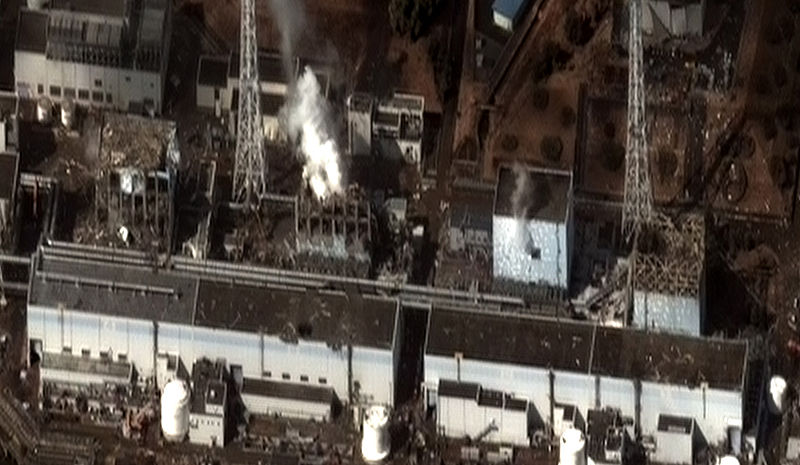
\includegraphics[scale=0.4]{./graph/800px-Fukushima_I_by_Digital_Globe.jpg}};
\node at (0,-3.5) {\tiny Source: Wikimedia Commons, \url{http://commons.wikimedia.org/wiki/File:Fukushima_I_by_Digital_Globe.jpg}};
}
\uncover<2->{
%\draw[white,fill=white] (-5,1) rectangle (5,3);
\node at (0,2.6) {\parbox{\textwidth}{
 \begin{alertblock}{common-cause failure} 
 \emph{simultaneous failure of several redundant components\\ due to a common or shared root cause}
 (H{\o}yland \& Rausand, 1994)
 \end{alertblock}
}};
}
\uncover<3>{
\draw[white,fill=white] (-0.2,-3.3) rectangle (6,0.75);
\node at (3,-1) {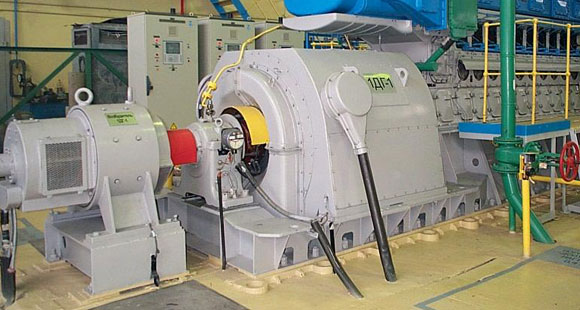
\includegraphics[scale=0.3]{./graph/plant-systems-diesel-generator.jpg}};
\node at (3.05,-3.05) {\parbox{6.2cm}{\tiny Source: \url{http://www.diakont.com/solutions/nuclear-energy/plant-systems/diesel-generator-control-systems/}}};
}
\end{tikzpicture}

% Notes for the slide
\note<3>[item]{All 12 generators (for 6 reactors) at Fukushima Daiichi\\ were not available due to flooding of machine rooms\\
 (Tsunami caused by T\={o}hoku earthquake)}
\note<3>[item]{Reliability of redundant systems}
\note<3>[item]{Usually 2 -- 4 emergency diesel generators per reactor}
\note<3>[item]{Sufficient cooling of core if one generator works}
\note<3>[item]{Reliability through redundancy is jeopardised by common-cause failure:}
\note<3>[item]{Redundant components may not fail independently: common-cause failure}
\note<3>[item]{Must include common-cause failures in overall system reliability analysis}
}

\frame{
\frametitle{Common-Cause Failure Modelling ***raus?}

\begin{columns}%[T]
\begin{column}{0.7\textwidth}\centering
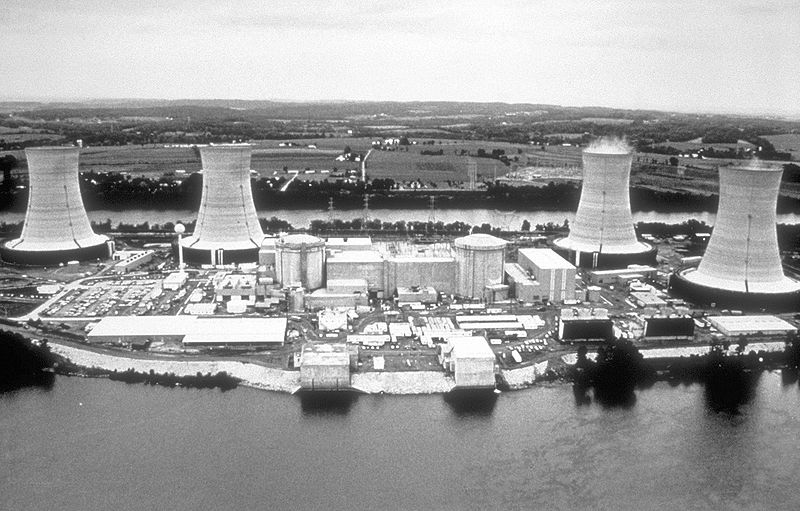
\includegraphics[scale=1.2]{./graph/800px-Three_Mile_Island_nuclear_power_plant.jpg}
\end{column}
\begin{column}{0.35\textwidth}\centering
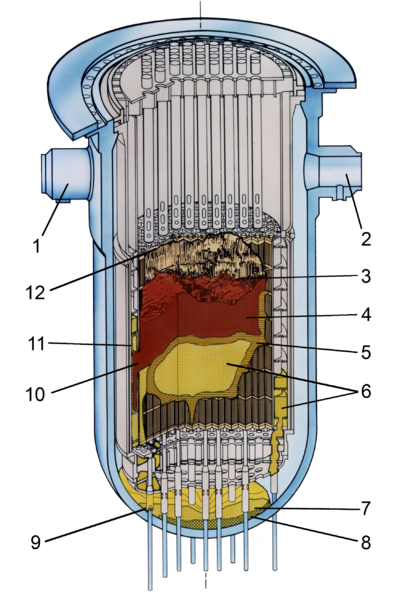
\includegraphics[scale=0.95]{./graph/Graphic_TMI-2_Core_End-State_Configuration.png}
\end{column}
\end{columns}
\vspace*{1ex}
\begin{tiny}
Above: CDC, \url{http://phil.cdc.gov/phil/} ID 1194\\[1ex]
Right: Wikimedia Commons,\\[-1.8ex]
\url{http://commons.wikimedia.org/wiki/File:Graphic_TMI-2_Core_End-State_Configuration.png}
\end{tiny}
% Notes for the slide
\note<1>[item]{Lesson learned at another accident: Three Mile Island (1979) where also a meltdown happened (right)}
\note<1>[item]{Most popular model: \emph{basic parameter model}, we will look at a parameterisation of it called\ldots}
}

\subsection{Alpha-Factor Model}

\begin{frame}{Alpha-Factor Model: Definition}
  \begin{block}{Alpha-Factor Model} %\cite{1988:mosleh::common:cause}]
    Multinomial distribution $\mult(\vec{n}\mid\vec{\alpha})$ for common-cause failures \\
    in a $k$-component system\vspace*{-2ex}
    %the number of redundant components in the common-cause component group
    \begin{align*}
      p(\vec{n}\mid\vec{\alpha})=\prod_{j=1}^k\alpha_j^{n_j}\\[-5ex]
    \end{align*}
    where
    \begin{itemize}
    \item \alert{alpha-factor}
      $\alpha_j\coloneqq$
      \parbox[t]{0.6\textwidth}{%
        probability of $j$ of the $k$ components \\
        failing due to a common cause \\
        given that failure occurs
      }
    \item \alert{failure count}
      $n_j\coloneqq$ corresponding number of failures observed
    \item $\vec{n}$ denotes $(n_1,\dots,n_k)$ and $\vec{\alpha}$ denotes $(\alpha_1,\dots,\alpha_k)$
    \end{itemize}
  \end{block}
  (the model actually serves to estimate failure \emph{rates},\\ but the above is all what matters in this talk)
\note<1>[item]{Slide on inferences in alph-factor model commented out}
\end{frame}

\iffalse
\begin{frame}{Alpha-Factor Model: Inference}
  \begin{block}{Inference}
    involves rational functions \\
    of probabilities $\vec{\alpha}$ of common-cause failures\\
    and of total failure rate $q_t$ for individual components
  \end{block}
  \begin{center}
    \textbf{this talk: focus on $\vec{\alpha}$ only}
  \end{center}
\end{frame}
\fi

\begin{frame}{Alpha-Factor Model: Parameter Estimation}

%\begin{itemize}
maximum likelihood estimator: 
    \begin{align*}
      \hat{\alpha}_j &= \frac{n_j}{n},\quad \text{where $\textstyle\sum_{j=1}^n n_j = n$}
    \end{align*}
%\end{itemize}

\uncover<2->{%
  \begin{alertblock}{The Problem}%{The Bad News}
    \begin{itemize}[<+->]
    \item typically, for $j\ge 2$, the $n_j$ are very low \\
      with zero being quite common for larger $j$
    \item zero counts = flat likelihoods \quad\then\quad $\hat{\alpha}_j =$?
%      standard techniques such as MLE can struggle \\
%      to produce sensible inferences for this problem
%    \item need to rely on \alert{epistemic information}\\
%       \quad \then\ Bayesian inference
    \end{itemize}
  \end{alertblock}}
\uncover<3->{%
  \begin{center}
    \textbf{\then\ need to rely on \alert{epistemic information}: Bayesian inference}
  \end{center}}
\end{frame}


\subsection{Bayesian Inference}

\begin{frame}{Bayesian Inference: Dirichlet Prior}
\uncover<1->{%
  $\vec{\alpha}$ considered as uncertain parameter on which we put\dots
  \begin{block}{Dirichlet Distribution ($\to$ Dirichlet-Multinomial Model)}
  \begin{columns}
  \begin{column}{0.65\textwidth}
    \begin{align*}
      p(\vec{\alpha}\mid \nzg,\byzr) \propto \prod_{j=1}^k\alpha_j^{\nzg\yzjr-1}
    \end{align*}
  \end{column}  
  \begin{column}{0.35\textwidth}
    \rule{0ex}{3ex}where $(\nzg, \byzr)$\\ are \emph{hyperparameters}
 \end{column}
 \end{columns}\vspace*{-1.8ex}
    \begin{align*}
      \nzg &> 0\\[-1ex]
      \byzr &\in \Delta=\Big\{
        (\yzor,\dots,\yzkr)\colon \yzor\ge0,\dots,\yzkr\ge 0,\,\sum_{j=1}^k \yzjr=1
      \Big\}
    \end{align*}
  \end{block}}
\uncover<2->{%
  \vspace*{-0.5ex}
  \begin{block}{Interpretation}
    \begin{itemize}
    \item $\byzr$ = \alert{prior expectation of $\vec{\alpha}$}, i.e., a prior guess for $\frac{n_j}{n}$, $j=1,\ldots,n$
    \item $\nzg$ = determines \alert{spread} and \alert{learning speed} (see next slide)
    \end{itemize}
  \end{block}}
\note<1>[item]{draw 1d and 2d simplex on black board}
\end{frame}

\begin{frame}{Bayesian Inference: Dirichlet Posterior}
  \begin{itemize}[<+->]
  \item posterior density for $\vec{\alpha}$ is again Dirichlet \ \ \then\ \ \alert{conjugacy}\\
  \alert{update parameters}: $\nzg \to\ \nng$, $\byzr \to \bynr$
    \begin{align*}
      p(\vec{\alpha}\mid\nzg,\byzr,\vec{n})
      &=
      p(\vec{\alpha}\mid\nng,\bynr)
      \propto
%      \prod_{j=1}^k\alpha_j^{\nzg\yzjr+n_j-1}
      \prod_{j=1}^k\alpha_j^{\nng\ynjr-1}
    \end{align*}
\item posterior expectation of $\alpha_j$:
    \begin{align*}
      %\label{eq:dirichlet:posterior:predictive}
      %\colorbox{red!10!white}{$\displaystyle
      \E[\alpha_j\mid\nzg,\byzr,\vec{n}]
      &=
      \E[\alpha_j\mid\nng,\bynr] 
      =
      \int_{\Delta}\alpha_j p(\vec{\alpha}\mid\nzg,\byzr,\vec{n})\dd\vec{\alpha} \\
      &= \ynjr
      =
      %\frac{n_j+st_j}{N+s}
      %=
      %\textcolor{green!50!black}{\frac{N}{N+s}}
      %\textcolor{blue}{\frac{n_j}{N}}
      %+
      %\textcolor{green!50!black}{\frac{s}{N+s}}
      %\textcolor{blue}{t_j}
      \colorbox{lmugreen!10!white}{$\displaystyle
      \frac{\nzg}{\nzg+n} \cdot \yzjr + \frac{n}{\nzg+n} \cdot \frac{n_j}{n}
      $}
    \end{align*}
%    where $n=\sum_{j=1}^k n_j$ is total number of observations
  \end{itemize}
  %\vspace{1em}
  \uncover<3->{%
%   \begin{alertblock}{}%{we will focus on $\E[\alpha_j\mid\nng,\bynr]$}
  \begin{center}
    \textbf{we will focus on $\E[\alpha_j\mid\nng,\bynr]$} \\
    (in a decision context, this expectation would typically end up \\
    in expressions for expected utility)
  \end{center}}
%   \end{alertblock}}
\end{frame}

\begin{frame}{Example: Prior and Data}
  (taken from Kelly \& Atwood, 2011) %\cite{2011:kelly:atwood})

  \begin{example}
    Consider a system with four redundant components ($k=4$). \\
    %The probability of
    %$j$ out of $k$ common-cause failures, given that failure has happend,
    %was denoted by $\theta_j$.
    The analyst specifies
    the following prior expectation $\mu_{\text{spec},j}$
    for each $\alpha_j$:
    \begin{align*}
      %\label{eq:example:muspec}
      \mu_{\text{spec},1}&=0.950
      &
      \mu_{\text{spec},2}&=0.030
      &
      \mu_{\text{spec},3}&=0.015
      &
      \mu_{\text{spec},4}&=0.005
    \end{align*}
    We have 36 observations, in which 35 showed one component failing,
    and 1 showed two components failing:
    \begin{align*}
      n_1&=35
      &
      n_2&=1
      &
      n_3&=0
      &
      n_4&=0
    \end{align*}
  \end{example}
\end{frame}

\begin{frame}{Example: Non-Informative Priors}
  \alert{large variation in posterior under different non-informative***link priors}
  \begin{itemize}[<+->]
  \item with constrained maximum entropy prior\\ (Atwood, 1996; Kelly \& Atwood, 2011): %\cite{1996:atwood,2011:kelly:atwood}):
    \begin{align*}
      \E[\alpha_1\mid\nng,\bynr]&=0.967
      &
      \E[\alpha_2\mid\nng,\bynr]&=0.028
      \\
      \E[\alpha_3\mid\nng,\bynr]&=0.003
      &
      \E[\alpha_4\mid\nng,\bynr]&=0.001
    \end{align*}
  \item 
  with uniform prior ($\yzjr=0.25$ and $\nzg=4$):
  \begin{align*}
    \E[\alpha_1\mid\nng,\bynr]&=0.9
    &
    \E[\alpha_2\mid\nng,\bynr]&=0.05
    \\
    \E[\alpha_3\mid\nng,\bynr]&=0.025
    &
    \E[\alpha_4\mid\nng,\bynr]&=0.025
  \end{align*}
  \item
  with Jeffrey's prior ($\yzjr=0.25$ and $\nzg=2$):
  \begin{align*}
    \E[\alpha_1\mid\nng,\bynr]&=0.9342
    &
    \E[\alpha_2\mid\nng,\bynr]&=0.0395
    \\
    \E[\alpha_3\mid\nng,\bynr]&=0.0132
    &
    \E[\alpha_4\mid\nng,\bynr]&=0.0132
  \end{align*}
  \end{itemize}%
% The degree of variation in the posterior under different priors
  % is evidently somewhat alarming.
  % In the next section, we aim to robustify the model
  % by using sets of priors from the start.
\note<1>[item]{emphasize variation for $\alpha_4$, the crucial part of the model\\
(all components fail): $0.1\%$ vs $2.5\%$ vs $1.3\%$}
\end{frame}

\subsection{Imprecise Dirichlet Model}

\begin{frame}{Imprecise Dirichlet Model: Definition}
\uncover<1->{%
Troffaes, Walter \& Kelly (2013): model vague prior info more cautiously
\begin{block}{Imprecise Dirichlet Model (IDM) for Common-Cause Failure}
use a \alert{set of hyperparameters}
    % \cite[p.~224, \S 5.4.3]{1991:walley} \cite[p.~32, \S 6]{1996:walley::idm},
    %\cite{1991:walley,1996:walley::idm}
    (Walley 1991, 1996):
    \begin{align*}
      %\label{eq:hyperparams:boxmodel}
      %\mathcal{H}
      \PZc
      =
      \left\{
        (\nzg,\byzr)
        \colon
        \nzg\in[\nzlg,\nzug],\,
        \byzr\in\Delta,\,
        \yzjr\in[\yzjlr{j},\yzjur{j}]
      \right\}
    \end{align*}
\end{block}\vspace*{-0.5ex}}\uncover<2->{%
\begin{block}{Interpretation}
\begin{itemize}
  \item we are doing a \alert{sensitivity analysis} (\'a la robust Bayes)\\ over $(\nzg,\byzr) \in \PZc$
  \item we take a \alert{set of priors} %$\text{conv}\big(\big\{p(\alpha\mid\nzg,\byzr) \colon (\nzg,\byzr) \in \PZc\big\}\big)$
  based on $\PZc$ \\
  as model for prior information (details later)
%  (resp.\ all convex mixtures of them)
\end{itemize}
\end{block}}\uncover<3>{%
Analyst has to specify (`elicit') \\
    bounds $[\nzlg,\nzug]$ and
    bounds $[\yzjlr{j},\yzjur{j}]$ for each $j\in\{1,\dots,k\}$ }%\\
\end{frame}

\begin{frame}{Imprecise Dirichlet Model: Elicitation}
  \begin{itemize}[<+->]
  \item   $[\yzjlr{j},\yzjur{j}]$: Cautious interpretation of prior specifications $\mu_{\text{spec},j}$:
  \begin{align*}
    [\yzjlr{1},\yzjur{1}]&=[0.950,1]
    &
    [\yzjlr{2},\yzjur{2}]&=[0,0.030]
    \\
    [\yzjlr{3},\yzjur{3}]&=[0,0.015]
    &
    [\yzjlr{4},\yzjur{4}]&=[0,0.005]
  \end{align*}
  \item  $[\nzlg,\nzug]$: Good (1965): \\ %\cite{1965:good}: \\
    \begin{center}
    reason about posterior expectations for hypothetical data
    \end{center}
  \end{itemize}
  \uncover<3->{%
  \begin{alertblock}{}
    $\nzug$ = number of one-component failures required \\
    to reduce the upper probabilities of multi-component failure by half
  \end{alertblock}
  \begin{alertblock}{}
    $\nzlg$ = number of multi-component failures required \\
    to reduce the lower probability of one-component failure by half
  \end{alertblock}}
\note<2>[item]{choice of bounds for $\nzg$ is not so straight-forward,
so we took advice from Good and reason about posterior expectations for hypothetical data,
also known as pre-posterior analysis}
\note<3>[item]{These rules are a bit difficult to grasp at first, so I'll explain them with the example:}
\end{frame}

\begin{frame}{Imprecise Dirichlet Model: Elicitation}
\uncover<1->{%
\begin{alertblock}{}
    $\nzug$ = number of one-component failures required \\
    to reduce the upper probabilities of multi-component failure by half
  \end{alertblock}
  \begin{alertblock}{}
    $\nzlg$ = number of multi-component failures required \\
    to reduce the lower probability of one-component failure by half
  \end{alertblock}}
  \uncover<2->{%
  Reasonable values in example:
  \begin{itemize}
  \item 
    $\nzug=10$: %\\
    after observing $10$ one-component failures \\
    \then\ halve upper probabilities of multi-component failures
  \item
    $\nzlg=1$: %\\
    immediate multi-component failure
    \\
    \then\ keen to reduce lower probability for one-component failure
  \end{itemize}}
  \uncover<3->{%
  \alert{Difference between $\nzlg$ and $\nzug$} reflects a \alert{level of caution}:\\
  The rate at which we reduce upper probabilities \\
  is less than the rate at which we reduce lower probabilities \\}
  %\then\ reflects a \alert{level of caution}
\end{frame}

\begin{frame}{Imprecise Dirichlet Model: Inference}
%  \begin{center}
%    prior bounds + likelihood $\to$ posterior bounds
%  \end{center}
%\vspace*{-2ex}
\begin{block}{prior bounds + likelihood $\to$ posterior bounds}
  \begin{center}
  \begin{tabular}{c|cc||cc}
    \multicolumn{1}{c}{}
  & \multicolumn{2}{c}{with $\yzjr=\mu_{\text{spec},j}$:}
  & \multicolumn{2}{c}{with bounds as earlier:} \\
    $j$ & $\El[\alpha_j\mid\PZc,\vec{n}]$ &$\Eu[\alpha_j\mid\PZc,\vec{n}]$
        & $\El[\alpha_j\mid\PZc,\vec{n}]$ &$\Eu[\alpha_j\mid\PZc,\vec{n}]$ \\
    \hline
    1 & 0.967\phantom{00} & 0.972\phantom{00} & 0.967\phantom{0} & 0.978\phantom{00}\\
    2 & 0.0278\phantom{0} & 0.0283\phantom{0} & 0.0270           & 0.0283\phantom{0}\\
    3 & 0.00041           & 0.00326           & 0\phantom{0.000}  & 0.00326\\
    4 & 0.00014           & 0.00109           & 0\phantom{0.000}  & 0.00109
  \end{tabular}
  \end{center}
\end{block} 
  \begin{itemize}%[<+->]
  \item<2-> \alert{Bounds}, rather than precise values, are desirable \\
    due to inferences being strongly sensitive to the prior \\
    particularly when faced with zero counts
  \item<3-> Simple ways to elicit the parameters of the model \\
    by \alert{reasoning on hypothetical data} \\
%    rather than by maximum entropy arguments
  \item<4-> Is it possible to generalise this method to other problems?
  \end{itemize}
\note<1>[item]{So what does this choice of parameter set mean for our number example?
We now have a posterior model that is based on a clear behavioural choice of prior,
expressing our prior ideas about $\vec{\alpha}$ and still being flexible enough to ***}
\end{frame}













\frame{\frametitle{Works the Thesis is Based on}

\nocite{Walter2009a-short,Walter2010a-long,Walter2011a,Walter2012b,Troffaes2013a-short,itip-statinf,luck-package}

\printbibliography[heading=none,keyword=defensethesis]

%\bibliographystyle{plainnat}
%\bibliography{../bib/eigene,../bib/itip-refs,../bib/other-refs}
}

\frame{\frametitle{Further References}

\nocite{1994:hoyland,1965:good,1991:walley,1996:walley::idm,2011:kelly:atwood,1996:atwood,2006:evans,2005:quaeghebeurcooman,1994:berger}

\printbibliography[heading=none,keyword=defensefurther]

%\bibliographystyle{plainnat}
%\bibliography{../bib/eigene,../bib/itip-refs,../bib/other-refs}
}



%---- Appendix: Updating and Mixture Commute

\begin{frame}[label=commute-app]{Updating and Mixture Commute \hyperlink{commute-back<3>}{\beamerreturnbutton{}}}

Let
\begin{align*}
p_m(\vartheta\mid \nz_1\!,\yz_1\!, \nz_2\!,\yz_2\!, \kappa) &:=
   \kappa\,  p(\vartheta\mid\nz_1\!,\yz_1) +
(1-\kappa)\, p(\vartheta\mid\nz_2\!,\yz_2) \,,
\end{align*}
with marginals
\begin{align*}
f_1(\x) &= \int_\Theta\! f(\x\mid\vartheta) p(\vartheta\mid \nz_1\!,\yz_1) \dd\vartheta \,, \\
f_2(\x) &= \int_\Theta\! f(\x\mid\vartheta) p(\vartheta\mid \nz_2\!,\yz_2) \dd\vartheta \,, \\
f_m(\x) &= \int_\Theta\! f(\x\mid\vartheta) p_m(\vartheta\mid \nz_1\!,\yz_1\!, \nz_2\!,\yz_2\!, \kappa) \dd\vartheta \\
        &=    \kappa  \int_\Theta f(\x\mid\vartheta) p(\vartheta\mid \nz_1\!,\yz_1) \dd\vartheta 
         + (1-\kappa) \int_\Theta f(\x\mid\vartheta) p(\vartheta\mid \nz_2\!,\yz_2) \dd\vartheta \\
%        &=    \kappa  \int_\Theta f_1(\x) p(\vartheta\mid \nn_1,\yn_1) \dd\vartheta 
%         + (1-\kappa) \int_\Theta f_2(\x) p(\vartheta\mid \nn_2,\yn_2) \dd\vartheta \\
        &= \kappa f_1(\x) + (1-\kappa) f_2(\x) \,.
\end{align*}

\end{frame}

\frame{\frametitle{Updating and Mixture Commute \hyperlink{commute-back<3>}{\beamerreturnbutton{}}}

%Then
\begin{align*}
\lefteqn{
p_m(\vartheta\mid \nz_1,\yz_1, \nz_2,\yz_2, \kappa, \x) } \hspace*{8ex} & \\[2ex]
 &= \frac{f(\x\mid\vartheta)}{f_m(\x)} \big(
     \kappa\,  p(\vartheta\mid\nz_1,\yz_1) +
  (1-\kappa)\, p(\vartheta\mid\nz_2,\yz_2) \big) \\
 &=  \kappa\,  \frac{f(\x\mid\vartheta) p(\vartheta\mid\nz_1,\yz_1)}{f_m(\x)} +
  (1-\kappa)\, \frac{f(\x\mid\vartheta) p(\vartheta\mid\nz_2,\yz_2)}{f_m(\x)} \\
 &=  \kappa\,  \frac{f_1(\x) p(\vartheta\mid\nn_1,\yn_1)}{f_m(\x)} +
  (1-\kappa)\, \frac{f_2(\x) p(\vartheta\mid\nn_2,\yn_2)}{f_m(\x)} \\
 &= p_m(\vartheta\mid \nn_1,\yn_1, \nn_2,\yn_2, \kappa^*)\,,
\end{align*}
\begin{align*}
\text{where}\hspace{5ex}
\kappa^* &= \kappa\, \frac{f_1(\x)}{f_m(\x)}
          = \frac{\kappa\, f_1(\x)}{\kappa\, f_1(\x) + (1-\kappa)\, f_2(\x)}\,. 
\end{align*}

}

\frame{\frametitle{Updating and Mixture Commute \hyperlink{commute-back<3>}{\beamerreturnbutton{}}}

\begin{itemize}
\item updated mixture distribution is a mixture of the updated components
with mixture parameter $\kappa^*$ instead of $\kappa$.
\item convex hull of prior components\\ $=$ set of prior mixture distributions with $\kappa \in [0,1]$.
\item for any $\kappa \in [0,1]$, the corresponding $\kappa^* \in [0,1]$.
\item in fact, $\{\kappa^* \mid \kappa \in [0,1]\} = [0,1]$.
\item set of updated mixture distributions with $\kappa^* \in [0,1]$\\ $=$ convex hull of updated components.
\item arbitrary number of components by complete induction.
\end{itemize}
}


%---- Appendix: reset total frame number
\addtocounter{framenumber}{-3} 

\end{document}
